\section{Uživatelské činnosti}

\subsection{Uživatelské role}

Z funkčních požadavků plyne, že každý uživatel v systému má vždy přiřazenou právě jednu z globálních rolí. Tím se stanovují jejich práva na provádění určitých činností v rámci \gls{is}.

Základní množinu uživatelských rolí tvoří \texttt{administrator}, \texttt{banned}, \texttt{user}, \texttt{authority} a imaginární role \texttt{guest}, jež se přímo nevyskytuje v \gls{is} a pouze označuje neautorizované osoby. Diagram na obrázku \ref{pic:dia-actors-global} znázorňuje logickou dědičnost těchto rolí na základě přístupových práv. Administrátor (\texttt{administrator}) systému má povolené všechny typy činností, zablokovanému (\texttt{banned}) uživateli je povoleno pouze přihlášení a přehled soukromých dat. Přístupová práva ostatních rolí jsou smíšená a jsou podrobně definována v seznamu případů užití.


\begin{fig:illustration}
   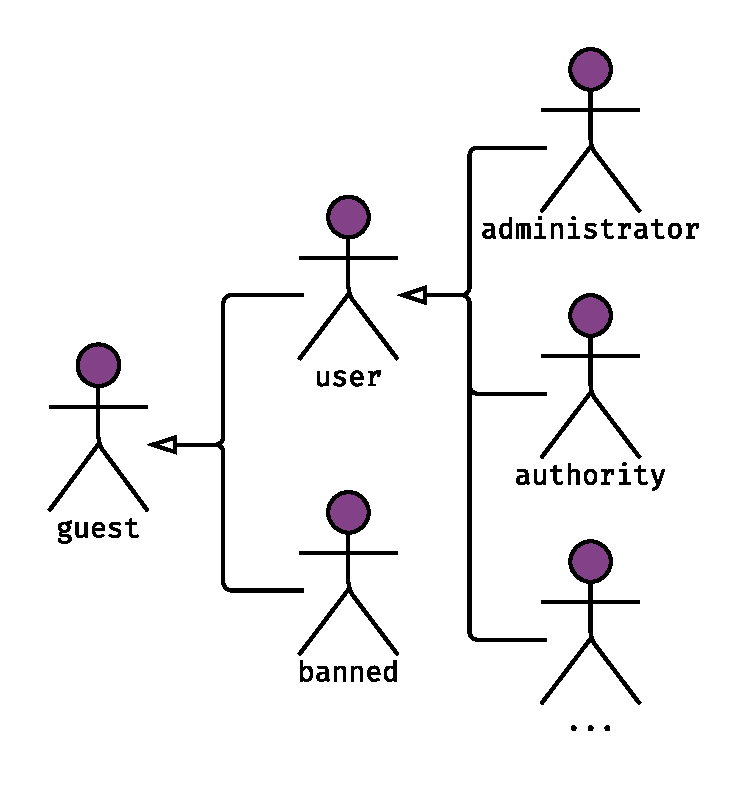
\includegraphics[width=0.5\textwidth]{images/dia-actors-global.pdf}
   \caption{Diagram logické dědičnosti globálních uživatelských rolí v systému}\label{pic:dia-actors-global}
\end{fig:illustration}


V každém projektu uživatelé budou nabývat sekundárních rolí, jež budou mít vliv pouze na daný projekt. Mezi ně patří vedoucí projektu (\texttt{leader}), skupina uživatelsky definovaných rolí spolupracovníků (\texttt{contributor}) a návštěvníci (\texttt{visitor}) s právy pouze pro čtení. Jejich logická dědičnost je znázorněna ve formě diagramu na~obrázku~\ref{pic:dia-actors-project}.


\begin{fig:illustration}
   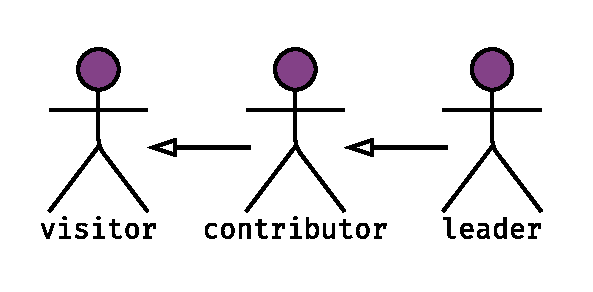
\includegraphics[width=0.5\textwidth]{images/dia-actors-project.pdf}
   \caption{Diagram logické dědičnosti uživatelských rolí v projektu}\label{pic:dia-actors-project}
\end{fig:illustration}



\subsection{Případy užití}

Případ užití neboli \gls{uc} je činnost, k vykonávání které dochází ze strany uživatele \gls{is} (buď člověka nebo jiného systému). Jednotlivé činnosti jsou řazeny do~dříve definovaných funkčních požadavků a během implementování jsou přímo promítány na jednotlivé typy oprávnění, jež budou přiřazovány globálním a projektovým rolím.


\begin{dlnar}
   \item[FR00] \textbf{Identita uživatelů}

   \begin{dlnar}
      \item[UC00]
      \texttt{guest} se může zaregistrovat nebo přihlásit do \gls{is}.
   \end{dlnar}
\end{dlnar}



\begin{dlnar}
   \item[FR01] \textbf{Globální role}

   \begin{dlnar}
      \item[UC01] 
      \texttt{administrator} může měnit roli uživatele. 
   \end{dlnar}
\end{dlnar}


\begin{dlnar}
   \item[FR02] \textbf{Osobní informace uživatelů}
 
   \begin{dlnar}
      \item[UC02] 
      Jakýkoliv účastník \gls{is} může prohlédnout svoje osobní informace. 

      \item[UC03] 
      Jakýkoliv účastník \gls{is} může odstranit svůj účet.
   \end{dlnar}
\end{dlnar}


\begin{dlnar}
   \item[FR03] \textbf{Upozornění}
 
   \begin{dlnar}
      \item[UC04] 
      \texttt{user} může zobrazit, upravit stav nebo odstranit svoje upozornění.
   \end{dlnar}
\end{dlnar}


\begin{dlnar}
   \item[FR04] \textbf{Projekt -- Životní cyklus}
   
   \begin{dlnar}
      \item[UC05]
      \texttt{user} může založit projekt. 

      \item[UC06]
      \texttt{user} s projektovou rolí \texttt{leader} může odstranit projekt. 

      \item[UC07]
      \texttt{user} s projektovou rolí \texttt{leader} může nastavit stav archivace.
   \end{dlnar}
\end{dlnar}


\begin{dlnar}
   \item[FR05] \textbf{Projekt -- Správa dat}
   
   \begin{dlnar}
      \item[UC08]
      \texttt{user} s projektovou rolí \texttt{leader} může upravit veřejné informace a interní popis projektu.
   \end{dlnar}
\end{dlnar}


\begin{dlnar}
   \item[FR06] \textbf{Projekt -- Kategorie a tagy}
 
   \begin{dlnar}
      \item[UC09]
      \texttt{user} s projektovou rolí \texttt{leader} může přidávat, upravovat a odstranovat tagy projektu. 

      \item[UC10]
      \texttt{authority} může zakládat, upravovat a odstranovat kategorie, pokud neobsahuje ani jeden projekt. 
   \end{dlnar}
\end{dlnar}


\begin{dlnar}
   \item[FR07] \textbf{Projekt -- Tým a role}
 
   \begin{dlnar}

      \item[UC11] 
      \texttt{user} s projektovou rolí \texttt{leader} může přidávat, upravovat a odstraňovat projektové role typu \texttt{contributor}.

      \item[UC12]
      \texttt{authority} s projektovou rolí \texttt{leader} může přidávat uživatelé do týmu.

      \item[UC13] 
      \texttt{user} s projektovou rolí \texttt{leader} může měnit projektovou roli uživatele.

      \item[UC14]
      \texttt{user} s projektovou rolí \texttt{leader} může odstraňovat uživatelé z týmu.

      \item[UC15] 
      \texttt{user} s projektovou rolí \texttt{leader} může povolovat nebo zakazovat volné přihlášení do projektové role \texttt{visitor} a rolí typu \texttt{contributor}.

      \item[UC16]
      \texttt{user} se může hlásit na vakantní místo.
   \end{dlnar}
\end{dlnar}


\begin{dlnar}
   \item[FR08] \textbf{Projekt -- Vyhledávání}
   
   \begin{dlnar}
      \item[UC17] 
      \texttt{user} může vyhledat projekt, pokud je projekt zařazen do seznamu pro vyhledávání.

      \item[UC18]
      \texttt{user} s projektovou rolí \texttt{leader} může přidávat nebo odebírat projekt ze~seznamu pro vyhledávání.
   \end{dlnar}
\end{dlnar}


\begin{dlnar}
   \item[FR09] \textbf{Projekt -- Iterace a úkoly}
   
   \begin{dlnar}
      \item[UC19] 
      \texttt{user} s projektovou rolí \texttt{leader} může přidávat, upravovat a odstraňovat iterace a úkoly.
   \end{dlnar}
\end{dlnar}


\begin{dlnar}
   \item[FR10] \textbf{Projekt -- Správa obsahu}
 
   \begin{dlnar}
      \item[UC20] 
      \texttt{user} s projektovou rolí \texttt{contributor} může přiřazovat části obsahů úkolům.

      \item[UC21] 
      \texttt{user} s projektovou rolí \texttt{contributor} může zakládat, upravovat a odstraňovat části v obsahu. 

      \item[UC22] 
      \texttt{user} s projektovou rolí \texttt{visitor} může zobrazit obsah.
   \end{dlnar}
\end{dlnar}


\begin{dlnar}
   \item[FR11] \textbf{Projekt -- Snímky iterací}
 
   \begin{dlnar}
      \item[UC23]
      \texttt{user} s projektovou rolí \texttt{contributor} projektu může vytvořit snímek.

      \item[UC24] 
      \texttt{user} s projektovou rolí \texttt{visitor} projektu může zobrazit snímek.

      \item[UC25] 
      \texttt{user} s projektovou rolí \texttt{contributor} projektu může odevzdat snímek.

      \item[UC26]
      \texttt{authority} s projektovou rolí \texttt{leader} může ohodnotit snímek, pokud je odevzdaný.
      
      \item[UC27]
      \texttt{authority} s projektovou rolí \texttt{leader} může změnit hodnocení snímku, pokud je jeho hodnotitelem.

      \item[UC28]
      \texttt{user} s projektovou rolí \texttt{leader} může odstranit snímek, pokud nebyl ohodnocen.  
   \end{dlnar}
\end{dlnar}
